 \documentclass[conference]{IEEEtran}
\IEEEoverridecommandlockouts
% The preceding line is only needed to identify funding in the first footnote. If that is unneeded, please comment it out.

\usepackage{amsmath,amssymb,amsfonts}
\usepackage{algorithmic}
\usepackage{pdfpages}
\usepackage{graphicx}
\usepackage{datetime}
\usepackage{braket}
\usepackage{textcomp}
\usepackage[T1]{fontenc}
\usepackage{url}
\usepackage{xcolor}
\usepackage[utf8]{inputenc}
\usepackage[english]{babel}
\usepackage[hidelinks,colorlinks=true,linkcolor=blue,citecolor=blue]{hyperref}
\usepackage{csquotes}
\DeclareMathAlphabet\mathrsfso      {U}{rsfso}{m}{n}
\def\BibTeX{{\rm B\kern-.05em{\sc i\kern-.025em b}\kern-.08em
    T\kern-.1667em\lower.7ex\hbox{E}\kern-.125emX}}


\usepackage[
backend=biber,
style=numeric,
sorting=none
]{biblatex}
\addbibresource{references.bib}
\pagestyle{plain}
\pagenumbering{arabic}

\begin{document}
\title{Heisenberg's Uncertainty Principle\\
%{\footnotesize \textsuperscript{} Write up PHY431}
%\thanks{Identify applicable funding agency here. If 
}

\author{\IEEEauthorblockN{Parivesh Choudhary}
\IEEEauthorblockA{%\textit{Department of Physics} \\
\textit{Department of Physics, Indian Institute of Technology Kanpur}\\
\textit{Kanpur, 208016, India}\\
\href{mailto:parivesh@iitk.ac.in}{parivesh@iitk.ac.in}}
\textit{(Dated: November 28 2020)}
}

\maketitle
\thispagestyle{plain}
\begin{abstract}

The Heisenberg’s Uncertainty Principle(HUP) was discovered by Werner Heisenberg in 1927. It is often misunderstood as the inability to measure certain properties of quantum objects exactly. This paper focuses on the real meaning of the Uncertainty Principle and how this principle is being used in Gravitational Wave astronomy.

\end{abstract}

%\begin{IEEEkeywords}
%component, formatting, style, styling, insert
%\end{IEEEkeywords}

\section{Introduction}
Music offers a good  example to explain the concept of uncertainty principle better: to calculate the precise pitch of the guitar string; the string must vibrate long enough to allow the measurement of the duration of the oscillation period. If we measure over a certain period of time, the exact time of the measurement would be difficult to define. This indicates that the measurement's precise moment in time and the exact pitch are mutually exclusive. The uncertainty principle for the musical notes can be given as(non-dimensionalized equation):

\begin{equation}
\Delta f \Delta t \geq {1} 
\end{equation}
i.e. (error in frequency)$\times$(time taken to measure frequency) is greater than $\frac{1}{2\pi}$\cite{Heisenbergs,Musicians}.

\subsection*{Heisenberg’s Uncertainty Principle in Quantum Mechanics}

In Quantum Mechanics, the energy of a photon is hf, where h is Planck's constant. Multiplying equation (1) with h on both sides gives Heisenberg's uncertainty principle for energy:

\begin{equation}
\Delta E \Delta t \geq \frac{h}{4\pi} 
\end{equation}

Similarly, the momentum of a photon is  given as $\frac{h}{\lambda}$ where $\lambda$ is the wavelength of the photon; therefore Heisenberg's uncertainty principle for momentum is given as:

\begin{equation}
\Delta p \Delta x \geq \frac{h}{4\pi} 
\end{equation}
The above equation tells that the position and momentum of a particle cannot be simultaneously measured with arbitrarily high precision. For example, take a case of an electron in Hydrogen atom: one cannot exactly measure the position of the electron which is at a distance of $r$ from the nucleus, because then the momentum of the electron will be zero, which contradicts the zero-point energy.

This relation is not related to the inability of the measuring instrument, but it arises from the wave properties of particle, which is inherent in nature.  

\section{Geometrical Derivation of HUP}
Let us consider a wave function given by state $\phi$ as:
\begin{equation}
\ket{\phi}=(\hat{x}+i\lambda\hat{p})\ket{\psi}  
\end{equation}
where $\hat{x}$, $\hat{p}$, $\lambda$ and $\ket{\psi}$ are position operator, momentum operator, arbitrary real number and arbitrary state respectively. For any $\lambda$ and $\ket{\psi}$ we have $\braket{\phi|\phi}\geq 0$. 

Therefore:
\begin{equation}
\braket{\phi|\phi}=\braket{\psi|\hat{x}^2|\psi}-i\lambda\braket{\psi|\hat{p}\hat{x}|\psi}+i\lambda\braket{\psi|\hat{x}\hat{p}|\psi}+\lambda^2\braket{\hat{p}^2}\geq 0 
\end{equation}

\begin{equation}
=\braket{\hat{p}^2}\lambda^2+\braket{i[\hat{x},\hat{p}]}\lambda+\braket{\hat{x}^2}\geq 0    
\end{equation}
The above equation can be written as:
\begin{equation}
\Delta p^2 \lambda^2 + \braket{i[\hat{x},\hat{p}]}\lambda + \Delta x^2 \geq 0    
\end{equation}
where $\Delta p$ and $\Delta x$ are the uncertainties in measuring $\hat{p}$ and $\hat{x}$ respectively. Equation 7 is similar to equation of parabola given as:

\begin{equation}
f(\lambda)=a\lambda^2 + b\lambda+c    
\end{equation}
The minimum value is at $\lambda_{min}=\frac{-b}{2a}$ which is $f(\lambda_{min})=c-\frac{b^2}{4a}$. Given $f(\lambda_{min}) \geq 0$, we obtain $ac\geq\frac{b^2}{4}$
Therefore:
\begin{equation}
\Delta x^2 \Delta p^2 \geq \frac{\braket{i[\hat{x},\hat{p}]}^2}{4}     
\end{equation}
The commutator relation of position and momentum is defined as: 
\begin{equation}
[\hat{x},\hat{p}]=i\hbar    
\end{equation}
where $\hbar$ is $\frac{h}{2\pi}$. Taking square root on both sides:
\begin{equation}
\Delta x \Delta p \geq \frac{\hbar}{2}    
\end{equation}

\subsection*{Generalized Uncertainty Principle}

The above derivation is for position and momentum operators. However, it can be generalized for any two observables(a,b), which can be shown as\cite{mmoore}:
\begin{equation}
\Delta a^2 \Delta b^2 \geq \frac{\braket{i[\hat{a},\hat{b}]}^2}{4}      
\end{equation}
i.e.
\begin{equation}
\Delta a \Delta b \geq \frac{|\braket{[\hat{a},\hat{b}]}|}{2}      
\end{equation}

\section{Quantum Squeezed Light}

The Uncertainty Principle applies not only to particles like atoms and electrons but also to light waves. We can think of light as a wave of oscillating electric and magnetic fields, which has an amplitude and a phase. Just as there must always be some uncertainty in the position and momentum of an electron, there must also be some uncertainty in the amplitude and phase of a light wave.

\subsubsection*{Uncertainty Principle in Electric field}
The electric field in terms of quadrature can be given as\cite{phdthesis_eric}:
\begin{equation}
E(t)=\sqrt{\frac{4\pi \hbar \omega_0}{Ac}}[a_1(t)\cos{\omega_0 t}+a_2(t)\sin{\omega_0 t}]    
\end{equation}
where a$_1$(t) and a$_2$(t) are Amplitude and Phase Quadrature respectively. The relation between and these two operators is given as:
\begin{equation}
\Delta a_{1}^2 \Delta a_{2}^2 \geq |\frac{1}{2i}\braket{[a_1,a_2]}|^2=\frac{1}{4}    
\end{equation}
Quantum squeezing is a technique in which one of the variables of the Uncertainty principle is 'squeezed' to reduce the noise in the observation, at the expense of increased noise in the conjugate variable.

\section{Uncertainty Principle and Gravitational Waves}

Gravitational Waves(GW) are perturbations in the space-time fabric, which is generally caused by massive objects; like colliding binary black holes, supernovae, neutron stars etc.

Laser Interferometer Gravitational-Wave Observatories (LIGO) which are capable of measuring the length of the order of $10^{-21}$m  are currently being used to detect these GW. The main source of noise in these detectors is the shot noise, which is mainly caused by random fluctuations of photons of high power laser\cite{Chu}. When light photons pass through these fluctuations, they're jostled a little. This makes the light beams shift somewhat out of phase. Imagine, a fleet of small boats sailing across a turbulent sea, and how hard it will be to hold them together. These random phase shifts can produce false GW signals. 
\subsection*{Squeezing at LIGO}

To improve this shot-noise limit, Quantum Squeezed Light is used. The noise in amplitude and phase form the two variable of the Uncertainty Principle. A phase squeezed laser light is injected in the interferometer. Therefore according to equation 15, phase noise is reduced, but on the other side, it certainly increases the noise in amplitude(Fig 1). This method has improved the sensitivity of the interferometer by 25$\%$\cite{6988398}.

\begin{figure}[htbp]
\centerline{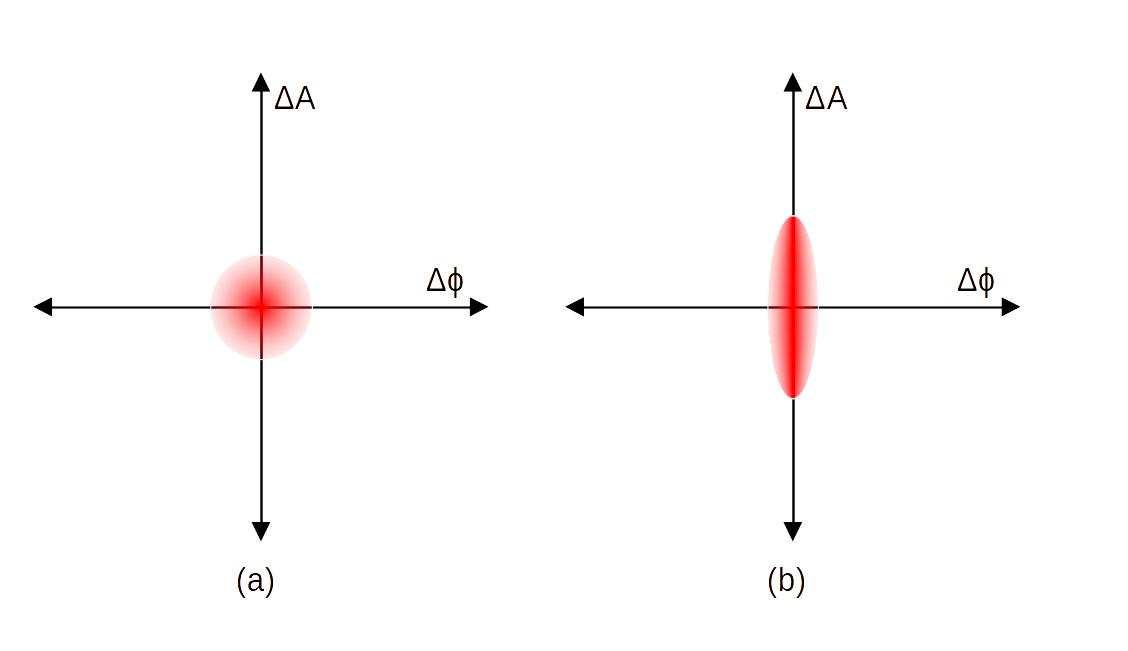
\includegraphics[scale=0.3]{Untitled_1.png}}
\caption{ (a) Quantum noise ‘ball’, showing the even distribution of uncertainty between the two quantities amplitude (A) and phase ($\phi$). (b) Squeezed noise, where the uncertainty in one quantity is less than quantum noise, while the other uncertainty is greater than quantum noise.}
\label{fig}
\end{figure}

\section{Conclusion}

The HUP is one of the most famous ideas in physics. Though, Albert Einstein firmly opposed to the theory of uncertainty, claiming that it could not actually represent reality, and spent several years debating with Heisenberg and others.The HUP is the heart of many things that we observe but cannot explain using classical physics. Werner Heisenberg's simple idea tells us why atoms do not implode, how the sun manages to shine and, that the vacuum of space is not actually empty. 


\section{References}
\printbibliography[heading=none]



\end{document}
